\section{Agentic Augmentation: Agent-Assisted Recommender Systems}
\label{sec:agent-assisted}

{Agent-assisted recommender systems insert an LLM agent \emph{around} a pre-existing recommendation pipeline to \textit{augment} specific sub-tasks (\eg retrieval/grounding, intent understanding, explanation, or constraint enforcement), while the core recommender remains the primary decision module.
In the language of autonomy, this category largely subsumes \textbf{L2 (retrieval-augmented)} and \textbf{L3 (tool-using)} systems: the agent improves the pipeline without fully replacing it, and the output is typically still anchored to classic recommendation primitives such as candidate generation and ranking.
This “assistance” framing matters because it changes what we optimize and what we measure: rather than asking whether an agent can recommend end-to-end, we ask which \emph{interventions} improve user and system outcomes, and how to evaluate those interventions reliably.}

{\paragraph{What tasks do agents assist with?}
Across the recent literature, agent-assisted systems repeatedly target a small set of recurring tasks, which can be grouped by \emph{where} they intervene in the recommendation loop:}

\begin{itemize}
    \item {\textbf{Understanding and control}: interpreting natural-language intent and constraints, eliciting missing preferences, and translating user commands into structured control signals (\eg conversational steering, controllable constraints) \cite{tang2025interactive,feng2025expectation,huang2025recommender,chen2025multi,zeng2024automated,luo2025rallrec+}.} 
    \item {\textbf{Grounding and knowledge access}: retrieving relevant information to reduce hallucinations and increase specificity (user-history snippets, item semantics such as attributes/reviews, external knowledge such as domain facts), typically via RAG-style components} \cite{tang2025interactive,feng2025expectation,huang2025recommender}. 
    \item {\textbf{Candidate operations and reranking}: generating candidate sets, filtering candidates under constraints, and reranking by richer semantic criteria (\eg compatibility reasoning or cross-domain transfer), often by coupling agents to RecTools \cite{zhao2024toolrec,yang2025agentdr,liu2025agentcf++,alamri2025leveraging}.} 
    \item {\textbf{Explanation and interaction quality}: producing grounded explanations and multi-turn justifications; summarizing rationales; clarifying trade-offs; adapting explanations to context \cite{sun2025retrieval,park2025madrec}.}
    \item {\textbf{Governance}: enforcing safety/fairness constraints, inserting intermediate representations or shields, and providing “guardrails” that sit between user, agent, and recommender \cite{xu2025iagent}; leveraging agent as engineer to update the recommendation strategies~\cite{lao2026agentx，wang2026self}.}
\end{itemize}

{Tasks often span multiple stages. For example, a multi-turn conversational assistant may (i) interpret an instruction, (ii) retrieve relevant history, (iii) call a ranking tool, and (iv) generate a justification; tool use and retrieval become \emph{mechanisms} that enable the task rather than ends in themselves.}

\subsection{Retrieval-Augmented Assistance}
\label{sec:assist-rag}


\begin{figure}[t]
% \vspace{-0.2cm}
\setlength{\abovecaptionskip}{0.02cm}
\setlength{\belowcaptionskip}{-0.3cm}
\centering
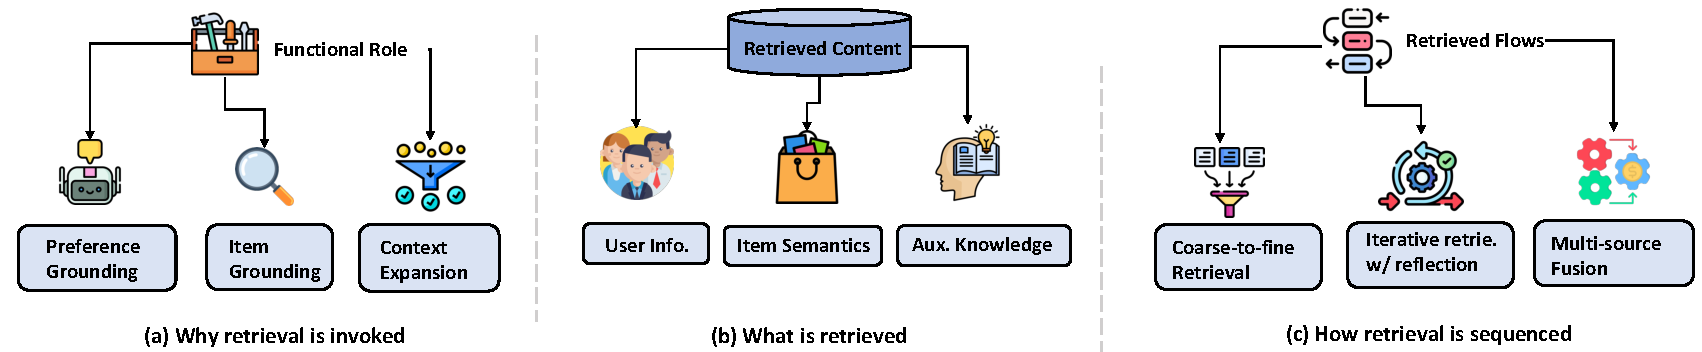
\includegraphics[width=0.99\linewidth]{figures/survey_r.pdf}
\caption{Illustration of three aspects of Retrieval-Augmented Assistance for Agent-assisted Recommender Systems.}
\label{fig:agent_assist_rag_tool_planning}
\end{figure}

{Retrieval augmentation is the dominant pattern for L2 systems and a key building block for L3 systems. While RAG is broadly used in NLP, in recommender systems the retrieved evidence must align with recommendation structure: it may contain \emph{user-side} information (profiles, histories, constraints), \emph{item-side} information (descriptions, reviews, attributes), or \emph{auxiliary knowledge} (domain facts, knowledge graphs, taxonomies).
Following the original survey’s framing, it is useful to organize retrieval-augmented recommendation through three complementary lenses: 

{{(i) \textbf{\textit{Functional role}}: why retrieval is invoked.}
Common functional roles include:
(1) \textbf{Preference grounding} (retrieve history snippets to ground intent and reduce inconsistency across turns). 
For example, RAH~\cite{shu2024rah} enhances the retrieval stage by querying a structured personality library to extract user-specific preferences, goals, and value orientations. These retrieved signals are then used to filter and prioritize candidate items, enabling more accurate and personalized candidate generation before downstream ranking.
iAgent~\cite{xu2025iagent} retrieves external knowledge through tool invocation while simultaneously leveraging the internal knowledge of LLMs, thereby assisting the reranker in further refining the ordering of an already ranked item list.
(2) \textbf{Item grounding} (retrieve item evidence to support explanations and avoid fabrication) \cite{kim2025itemrag,bhattacharya2025recbygen},
and (3) \textbf{Context expansion} (retrieve domain knowledge for niche domains such as health, finance, or travel) \cite{maragheh2025arag,borgeaud2022improving,zhao2025webrec,cho2025marc,banerjee2024enhancing, rao2024ramo}.
This perspective clarifies what “success” means: \eg for preference grounding we care about stability and faithfulness to user history, whereas for context expansion we care about factuality and usefulness.} 

{{(ii) \textbf{\textit{Retrieved content}}: what is retrieved.}
Retrieved content typically falls into:
\textbf{user information} (profiles, histories, constraints)~\cite{huang2024interecagent,shu2024rah,wang2024recmind,yu2025intelligent_agent,maragheh2025arag,kim2026leveraging, wei2025enhanced, ao2025retrieval, ning2026retrieval, yang2025retrieval}. 
User information is typically divided into long-term and short-term preferences and represented as interaction histories or textual preference evidence. 
For example, ARAG~\cite{maragheh2025arag} collects textual cues from both the current session and long-term logs to summarize user intent and support re-ranking. AgentCF~\cite{zhang2023agentcf} retrieves user memory and item memory to enrich preference representations and item semantics. AgentDR~\cite{yang2025agentdr} further incorporates tool-applicability memory, improving the automation level of agent-assisted recommendation. 
\textbf{item semantics} (attributes/reviews; multimodal content where available)~\cite{zhang2023agentcf,liu2025agentcf++,kim2025itemrag, wang2025knowledge, qiu2025graph, kieu2025keyword, li2025g, xu2025rallrec, yang2025cold,balachandran2025visiorag,wei2025learning}; for example, AgentCF~\cite{zhang2023agentcf} retrieves item memory to enrich item-side semantics, while AgentCF++~\cite{liu2025agentcf++} further leverages cross-domain semantic evidence to improve candidate understanding. 
and \textbf{auxiliary knowledge} (external corpora, KGs, or curated domain sources)  \cite{maragheh2025arag,xu2025iagent,borgeaud2022improving,meng2025balancing}; for example, iAgent~\cite{xu2025iagent} queries outside knowledge sources to refine reranking. 
This choice affects privacy and leakage risk: user-side retrieval often contains sensitive personal data, while auxiliary knowledge retrieval raises provenance and licensing issues.} 


{{(iii) \textbf{\textit{Retrieval flows}}: how retrieval is sequenced.}
Beyond “retrieve once then generate,” recent systems increasingly use multi-step flows, such as:
1) {coarse-to-fine retrieval} (retrieve broad candidates, then refine by constraints) \cite{huang2024interecagent,maragheh2025arag,li2025rallm},
2) {iterative retrieval with reflection} (retrieve, draft, detect missing evidence, retrieve again) \cite{huang2024interecagent,xu2025iagent,zhang2025sarrec},
or 3) {multi-source fusion} (combine user-history retrieval with item-attribute retrieval) \cite{zhang2023agentcf,liu2025agentcf++,zeng2024federated}.
These flows implicitly introduce \emph{planning} and should be evaluated at the trajectory level, not only by final accuracy.} 

{\paragraph{\textbf{Key limitations.}}
RAG-based assistance can still fail via (i) \emph{retrieval bias} (frequent or easy-to-retrieve patterns dominate), (ii) \emph{context overload} (critical evidence is “lost in the middle”), and (iii) \emph{spurious grounding} (retrieved text gives false confidence without causal relevance) \cite{maragheh2025arag,sun2025retrieval,xu2025iagent,liu2024lost,lichtenberg2024large,sun2025cirr,zhang2025customizedretrievalaugmentedgenerationllm, tandon2025evaluating, sayana2025beyond, lin2025strajrag, cheng2025education, meng2025kerag_r}.
These motivate evaluation protocols that explicitly test robustness to retrieval noise and long-context failure (Sec.~\ref{sec:evaluation}).  
Compared with conventional retrieval systems, retrieval-augmented recommender systems incorporate external behavioral traces and world knowledge into the recommendation process, thereby enhancing personalization and generalization. 
However, their autonomy remains limited: while they are able to integrate long-term context and historical memory to some extent, they still primarily operate reactively rather than proactively, rely on single-turn retrieval with limited interaction flexibility, and utilize fixed pipelines that are difficult to adapt. 
Thus, retrieval-augmented recommender systems can be regarded as a transitional stage bridging static retrieval models and autonomous recommendation agents capable of strategic reasoning, context-aware planning, and adaptive learning. 



\begin{table*}[!t]
\centering
\caption{Unified Summary of Retrieval-Augmented Assistance, Tool-Driven Assistance, and Planning as Assistance.}
\label{tab:unified_summary}
\resizebox{\textwidth}{!}{%
\begin{tabular}{p{2.5cm} p{3cm} p{3.5cm} p{5cm} p{5cm}}
\toprule
\textbf{Category} & \textbf{Dimension} & \textbf{Sub-type} & \textbf{Representative Works} & \textbf{High-level Capabilities} \\
\midrule

% =======================
% 1. Retrieval-Augmented Assistance
% =======================
\multirow{9}{=}{\textbf{Retrieval-Augmented Assistance}}

& \multirow{3}{=}{\textbf{Functional Role} \newline (Why retrieval is invoked)}
& Preference Grounding
& RAH~\cite{shu2024rah}, iAgent~\cite{xu2025iagent}
& \multirow{9}{=}{\textbf{Proactivity:} Reactive \newline
\textbf{Context Awareness:} Memory (long-/short-term) \newline
\textbf{Interaction:} Single-turn retrieval \newline
\textbf{Adaptivity:} Static pipeline} \\

& & Item Grounding
& AgentCF~\cite{zhang2023agentcf}, AgentCF++~\cite{liu2025agentcf++}
& \\

& & Context Expansion
& ARAG~\cite{maragheh2025arag}, iAgent~\cite{xu2025iagent}
& \\

\cmidrule{2-4}

& \multirow{3}{=}{\textbf{Retrieved Content} \newline (What is retrieved)}
& User Information
& InteRecAgent~\cite{huang2024interecagent}, RAH~\cite{shu2024rah}, RecMind~\cite{wang2024recmind}, ARAG~\cite{maragheh2025arag}, AgentCF~\cite{zhang2023agentcf}, AgentDR~\cite{yang2025agentdr}
& \\

& & Item Semantics
& AgentCF~\cite{zhang2023agentcf}, AgentCF++~\cite{liu2025agentcf++}
& \\

& & Auxiliary Knowledge
& ARAG~\cite{maragheh2025arag}, iAgent~\cite{xu2025iagent}
& \\

\cmidrule{2-4}

& \multirow{3}{=}{\textbf{Retrieval Flows} \newline (How retrieval is sequenced)}
& Coarse-to-Fine
& InteRecAgent~\cite{huang2024interecagent}, ARAG~\cite{maragheh2025arag}
& \\

& & Iterative with Reflection
& InteRecAgent~\cite{huang2024interecagent}, iAgent~\cite{xu2025iagent}
& \\

& & Multi-source Fusion
& AgentCF~\cite{zhang2023agentcf}, AgentCF++~\cite{liu2025agentcf++}
& \\

\midrule

% =======================
% 2. Tool-Driven Assistance
% =======================
\multirow{4}{=}{\textbf{Tool-Driven Assistance}}

& \multirow{4}{=}{\textbf{Tool Taxonomy} \newline (What tools are used)}
& RecTools
& InteRecAgent~\cite{huang2024interecagent}, ToolRec~\cite{zhao2024toolrec}
& \multirow{4}{=}{\textbf{Proactivity:} Proactive (tool invocation) \newline
\textbf{Context Awareness:} Internal \& external memory \newline
\textbf{Interaction:} Multi-turn \newline
\textbf{Adaptivity:} Adaptive strategy} \\

& & External Info Tools
& iAgent~\cite{xu2025iagent}, RecMind~\cite{wang2024recmind}
& \\

& & Attribute-oriented Tools
& ToolRec~\cite{zhao2024toolrec}
& \\

& & Multimodal Tools
& HuggingGPT~\cite{shen2023hugginggpt}, Toolformer~\cite{schick2023toolformer}
& \\[14pt]

\midrule

% =======================
% 3. Planning as Assistance
% =======================
\multirow{8}{=}{\textbf{Planning as Assistance}}

& \multirow{2}{=}{\textbf{Interaction} \newline \textbf{Planning}}
& Reflective Plan Revision
& InteRecAgent~\cite{huang2024interecagent}
& \multirow{8}{=}{\textbf{Planning:} Goal decomposition, tool orchestration \newline
\textbf{Reasoning:} Multi-step reasoning, reflection \newline
\textbf{Adaptivity:} Dynamic memory \& plan updates \newline
\textbf{Context Awareness:} Tools, history, interactions} \\

& & Expectation-driven Steering
& ECPO~\cite{feng2025expectation}
& \\[4pt]

\cmidrule{2-4}

& \multirow{2}{=}{\textbf{Representation} \newline \textbf{Planning}}
& Semantic Enrichment
& AgentCF~\cite{zhang2023agentcf}
& \\

& & Cross-domain Transfer
& AgentCF++~\cite{liu2025agentcf++}
& \\[4pt]

\cmidrule{2-4}

& \multirow{2}{=}{\textbf{Ranking/Reranking} \newline \textbf{Planning}}
& Reasoning-driven Reranking
& Intelligent Agent~\cite{yu2025intelligent_agent}
& \\

& & Reflective Learning
& Re2LLM~\cite{re2llm}, MoRE~\cite{more}, SRLF~\cite{srlf}, DRDT~\cite{drdt}
& \\

\bottomrule
\end{tabular}
}
\end{table*} 

\subsection{Tool-Driven Assistance}
\label{sec:assist-tools}

{Tool use is the hallmark of L3 systems: the agent does not merely condition on retrieved text, but \emph{acts} via API calls, database queries, retrieval services, rerankers, and other components.
In recommendation, tool use spans different stages, such as retrieval, ranking, and reranking. 
}

\paragraph{\textbf{Tool taxonomies and design choices.}}
A practical taxonomy separates:
(i) \textbf{RecTools} directly provides candidate sets or ranking lists (\eg traditional retrievers, rankers, candidate filters models); 
(ii) \textbf{external information tools} retrieve external knowledge and contextual signals (\eg web/domain search, knowledge base query tools); 
(iii) \textbf{attribute-oriented tools} filter items based on structured attributes or specific constraints (\eg feature calculators, KG completion, constraint checkers); 
and (iv) \textbf{multimodal tools} are used to understand multimodal features, or generate multimodal content to supplement recommendation tasks (\eg vision/audio encoders, captioners) \cite{zhao2024toolrec,huang2024interecagent,yang2025agentdr,shen2023hugginggpt,schick2023toolformer,shi2025ocgagent}. 
These tools can be invoked separately or sequentially in different contexts. 
For example, InteRecAgent~\cite{huang2024interecagent} calls recommendation tools to support task planning and execution, progressively refining the candidate pool before returning it to the LLM, which then delivers the final response to the user. 
In re-ranking, iAgent~\cite{xu2025iagent} queries external knowledge through search tools and forwards the retrieved information to a re-ranker to refine an already-ranked list. 
AgentDR exemplifies a tool-centric view where the agent learns to uncover implicit item--item relations by invoking a pipeline of tool operations, enabling dynamic recommendation under changing contexts \cite{yang2025agentdr}. 
{Tool selection policies can be hand-coded, prompted, or learned; recent work on modular ``hooks'' attempts to decouple tool invocation logic from prompts, improving maintainability and safety auditing \cite{de2024language}.
In practice, tool-driven assistance often succeeds not because the LLM is a strong ranker, but because it orchestrates structured components with better inductive bias (retrieval, ranking, graph search).


\subsection{Planning as Assistance}
\label{sec:assist-planning}

{Planning arises naturally once agents operate over multi-turn conversations and multi-step tool sequences. Importantly, planning is not only about conversation; it can appear in:
(1) \textbf{interaction planning} (\eg what to respond next, how to improve the recommendations) can be injected to decide what to ask next to the user, or be leveraged to generate intermediate plans to give guidance signals to improve recommender models that can align better with the user needs~\cite{huang2024interecagent,feng2025expectation}. 
(2) \textbf{Rrepresentation planning} (\eg what and how to update user preference and item descriptions) allows LLMs to construct richer, updated, and explainable user and item descriptions~\cite{zhang2023agentcf,liu2025agentcf++, xie2026agentictagger}.
(3) \textbf{Ranking/reranking planning} usually considers what constraints to satisfy first, or how to trade-off objectives, thus leading to a more constraint-compatible result that aligns with user preference at the same time~\cite{yu2025thought,yu2025intelligent_agent,shi2024large}.}
(4) \textbf{Optimization planning} leverages LLM agents to automatically diagnose algorithm limitations and update the recommendation strategies/pipelines iteratively~\cite{lao2026agentx,wang2026self}.

Existing literature has explored different types of planning to augment recommender systems. 
For example, InteRecAgent~\cite{huang2024interecagent} introduces explicit planning into the recommendation pipeline. 
By reflecting on user interactions, tool invocation plans, and intermediate recommendation outcomes, the agent continuously revises and optimizes its internal plans, thereby enhancing the system’s understanding of user intent and enabling more controllable and self-improving interactions. 
To enhance user/item representations, AgentCF~\cite{zhang2023agentcf} leverages automated user interaction histories and textual feedback to enrich the semantic representations of both users and items. By incorporating global collaborative information, it produces more comprehensive and fine-grained embeddings that offer a stronger foundation for downstream recommendation. In the ranking task, the Intelligent Agent~\cite{yu2025intelligent_agent} applies predefined reasoning rules to the pre-ranked list, performing step-by-step inference to assess whether each candidate item truly aligns with the user’s explicit or implicit preferences. This reasoning-driven refinement yields a more accurate and user-aligned final ranking than traditional scoring-based approaches.



{\paragraph{\textbf{Comparison between tool-driven and planning assistance (L3 $\rightarrow$ L4).}}
Compared with tool-driven agents, the single-agent planner stage exhibits stronger autonomy: it can actively set goals, break them into steps, and continuously observe, reflect, and adjust during execution; 
Together, these capabilities enable richer context awareness, proactive decision-making, flexible interaction, and continuous adaptivity, resulting in improved generalization and long-term recommendation performance.

